\documentclass{standalone}

\usepackage{tikz}

\tikzstyle{vertex}=[circle,draw=black!100,thick,minimum size=1cm]
\tikzstyle{pale_vertex}=[circle, draw=black!25!white, thick, minimum size=1cm]

\begin{document}
  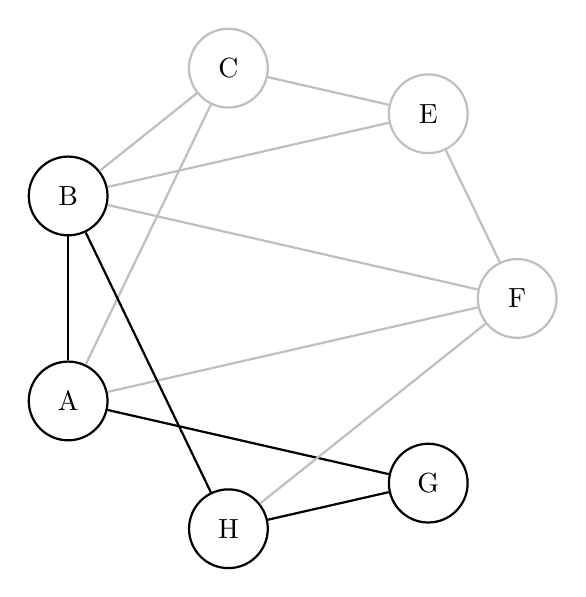
\begin{tikzpicture}
    \node (A) at (-2.7029066,  -1.30165122) [vertex] {A};
    \node (B) at (-2.7029066,   1.30165122) [vertex] {B};
    \node (C) at (-0.667562802, 2.92478374) [pale_vertex] {C};
    \node (E) at ( 1.87046941,  2.34549445) [pale_vertex] {E};
    \node (F) at (3,            0) [pale_vertex] {F};
    \node (G) at (1.87046941,   -2.34549445) [vertex] {G};
    \node (H) at (-0.667562802, -2.92478374) [vertex] {H};
    
    \draw (A) -- (B) [thick];
    \draw (A) -- (C) [thick, color=black!25!white];
    \draw (A) -- (F) [thick, color=black!25!white];
    \draw (A) -- (G) [thick];
    
    \draw (B) -- (C) [thick, color=black!25!white];
    \draw (B) -- (E) [thick, color=black!25!white];
    \draw (B) -- (F) [thick, color=black!25!white];
    \draw (B) -- (H) [thick];
    
    \draw (C) -- (E) [thick, color=black!25!white];
    
    \draw (E) -- (F) [thick, color=black!25!white];
    
    \draw (F) -- (H) [thick, color=black!25!white];
    
    \draw (G) -- (H) [thick];
  \end{tikzpicture}
\end{document}